\section{Performance Benchmarks}

When running the PETSc solvers on the CPU the following command line arguments
are given: "\emph{-vec\_type standard -mat\_type aij}". The matrix type
\emph{aij} is used for sparse matrices. When benchmarking with the PETSc solvers
on the GPU these command line arguments are given: "\emph{-vec\_type viennacl
-mat\_type aijviennacl}". The vector type \emph{viennacl} and matrix type
\emph{aijviennacl} use the ViennaCL library to perform calculations.

The configuration options for the wind simulator allows for variation in the
external wind direction, speed and the resolution of the three dimensional wind
velocity field. For the scope of these benchmarks only the resolution of the wind
velocity field is changed, while the external wind's speed and direction remains
unchanged for all benchmarks. The resolution of the wind velocity field is denoted
as \{x, y, z\}. The terrain used for the simulation benchmarks is the height map of
Mount St. Helens with a size of 768x768 that has been added by previous students
working on the snow simulator. The external wind's speed is set to 1 and the
direction is given by the unit vector \{1, 0, 0\}.

\subsection{Wind Simulation Benchmark}

In this benchmark the execution time of the wind simulation is measured as a
function of the resolution of the wind velocity field. The execution time of
the wind simulation is set to the average execution time of 100 frames of
simulation. This is done to account for noise in the execution time measurements.
The solver selected for this benchmark is GMRES, this was specified with the
command line argument "\emph{-ksp\_type gmres}".

For this benchmark the execution time of the wind simulation with PETSc with and
without GPU is measured. The execution time of the wind simulation previously
implemented in the snow simulator by other students is also measured to compare
with the PETSc implementation. The following configurations for the resolution of
the wind velocity field was used for this benchmark:

\begin{itemize}
	\item \{32, 16, 32\}
	\item \{32, 32, 32\}
	\item \{64, 32, 64\}
	\item \{64, 64, 64\}
	\item \{128, 64, 128\}
	\item \{128, 128, 128\}
	\item \{256, 128, 256\}
\end{itemize}

The total size of the wind field includes the external boundary points.

\begin{figure}[ht]
	\center
	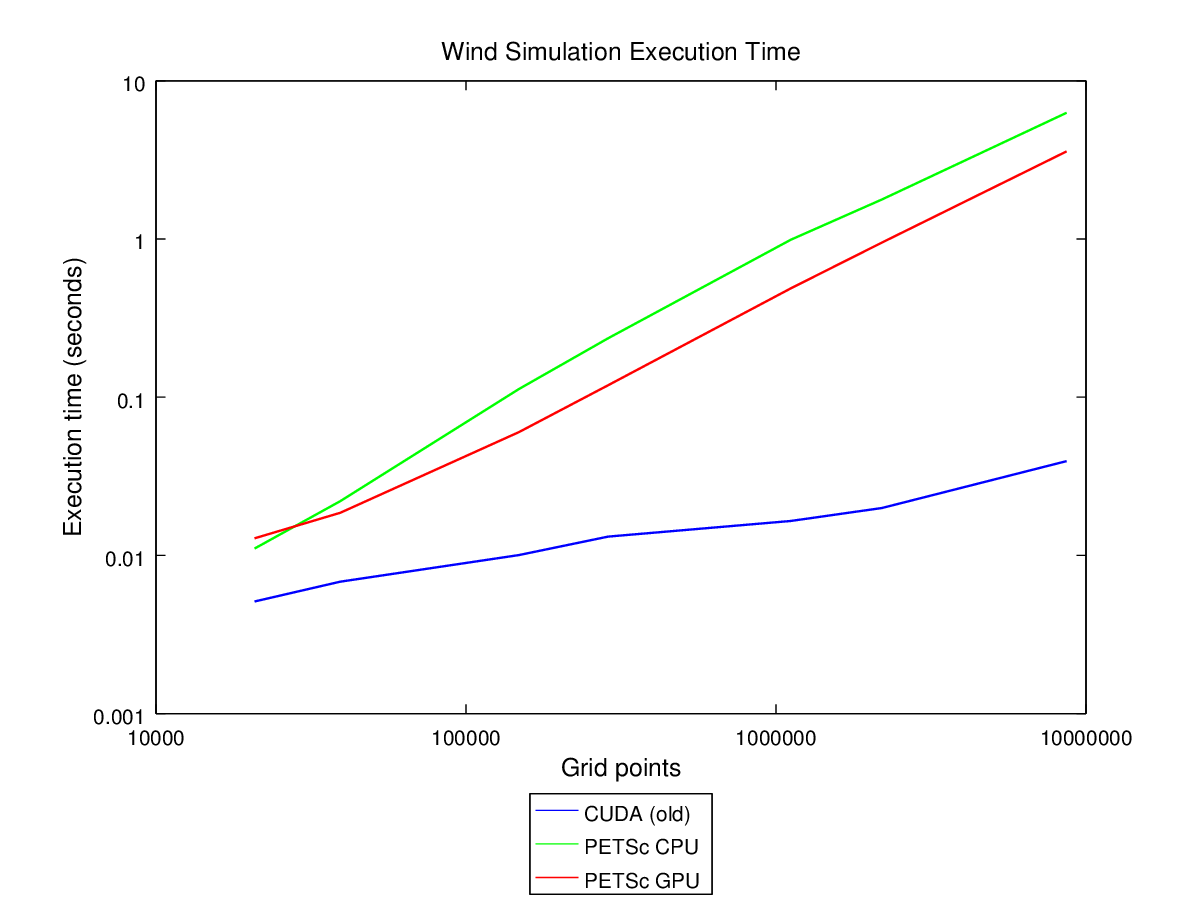
\includegraphics[width=1.0\textwidth]{results/data/wb/exec_time_all}
	\caption{Graph comparing the execution time for different wind simulator
		implementations.}
	\label{fig:wind_sim_time}
\end{figure}

TODO: 

\subsection{Compute Time Benchmark}

This benchmark measures how the execution time of the wind simulation is distributed
between these key functions in the implementation:
\begin{description}
	\item[advect:] Performs the advection step of the wind simulation.
	\item[setupSolution:] Computes the right-hand side of the linear system.
	\item[setInitialGuess:] Sets the initial guess for the solver.
	\item[solve:] Solves the Poisson equation using a PETSc solver.
	\item[project:] Performs the projection step of the wind simulation.
	\item[windToGPU:] Moves the wind velocity field to texture memory for the
	snow particle simulation.
\end{description}

The solver chosen for this benchmark is GMRES, specified with "\emph{-ksp\_type
gmres}".

This benchmark is performed for four different configurations for the resolution of
the wind velocity field:
\begin{description}
	\item[Configuration 1] $ \{ 32, 16, 32 \} $, results are shown in figure
		\ref{fig:td_conf1}.
	\item[Configuration 2] $ \{ 64, 32, 64 \} $, results are shown in figure
		\ref{fig:td_conf2}.
	\item[Configuration 3] $ \{ 128, 64, 128 \} $, results are shown in figure
		\ref{fig:td_conf3}.
	\item[Configuration 4] $ \{ 256, 128, 256 \} $, results are shown in figure
		\ref{fig:td_conf4}.
\end{description}

The results for the compute time benchmark is the average execution time of each
key function after 100 frames of simulation.

\begin{figure}[ht]
	\center
	
	\begin{subfigure}{0.45\textwidth}
		\center
		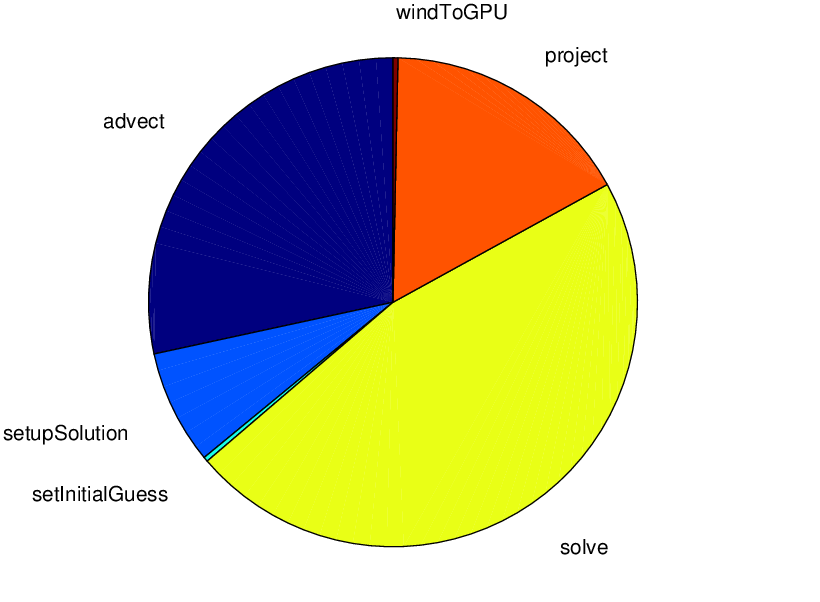
\includegraphics[width=1.0\textwidth]{results/data/td/td_conf1_petsc_gpu}
		\caption{PETSc on the GPU with OpenCL.}
		\label{fig:td_conf1_petsc_gpu}
	\end{subfigure}
	\begin{subfigure}{0.45\textwidth}
		\center
		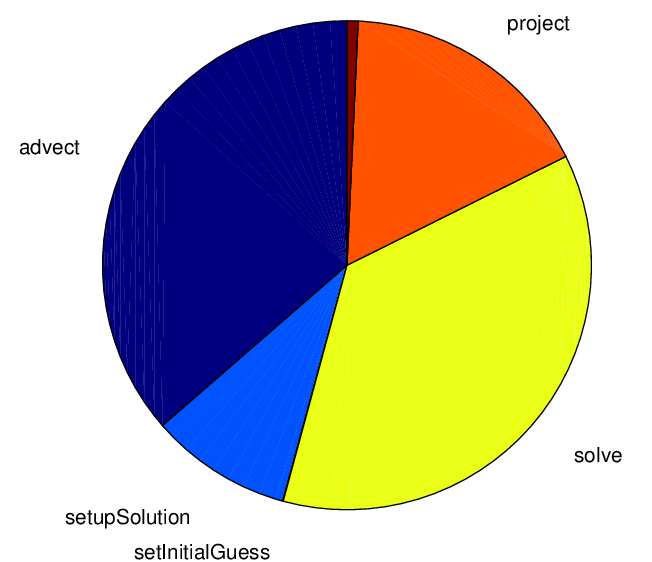
\includegraphics[width=1.0\textwidth]{results/data/td/td_conf1_petsc_cpu}
		\caption{PETSc on the CPU.}
		\label{fig:td_conf1_petsc_cpu}
	\end{subfigure}
	\caption{Compute time benchmark of the execution time of the key functions
			with configuration 1}
	\label{fig:td_conf1}
	
\end{figure}

\begin{figure}[ht]
	\center
	
	\begin{subfigure}{0.45\textwidth}
		\center
		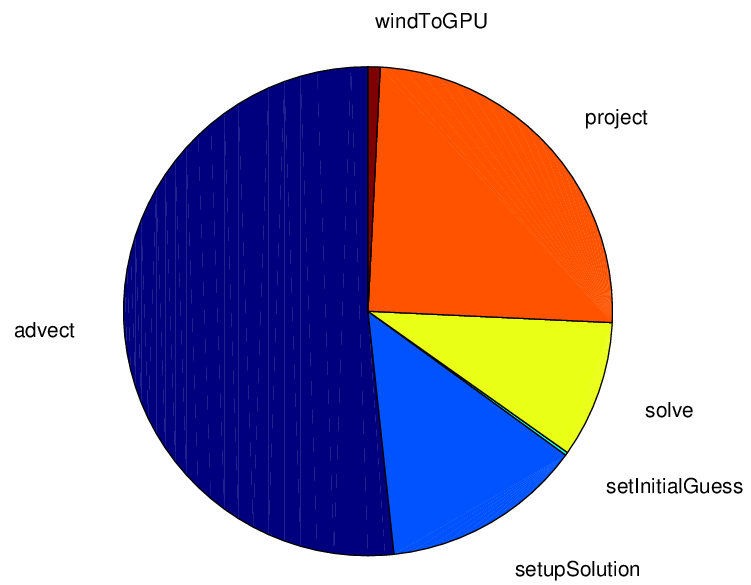
\includegraphics[width=1.0\textwidth]{results/data/td/td_conf2_petsc_gpu}
		\caption{PETSc on the GPU with OpenCL.}
		\label{fig:td_conf2_petsc_gpu}
	\end{subfigure}
	\begin{subfigure}{0.45\textwidth}
		\center
		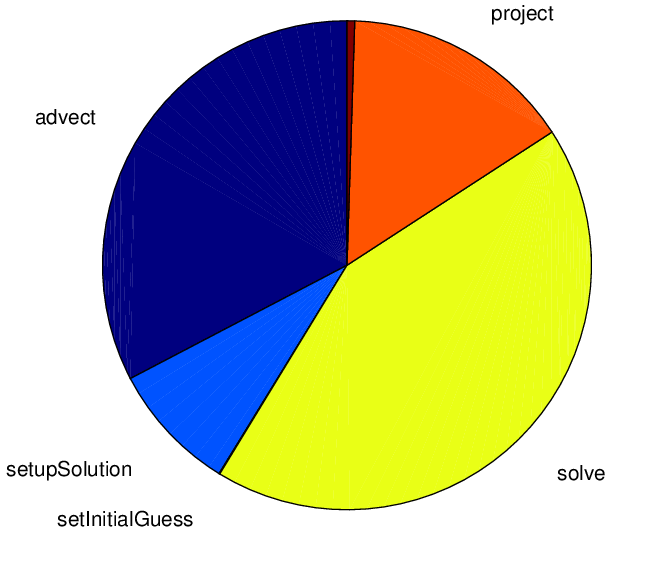
\includegraphics[width=1.0\textwidth]{results/data/td/td_conf2_petsc_cpu}
		\caption{PETSc on the CPU.}
		\label{fig:td_conf2_petsc_cpu}
	\end{subfigure}
	\caption{Compute time benchmark of the execution time of the key functions
			with configuration 2}
	\label{fig:td_conf2}
	
\end{figure}

\begin{figure}[ht]
	\center
	
	\begin{subfigure}{0.45\textwidth}
		\center
		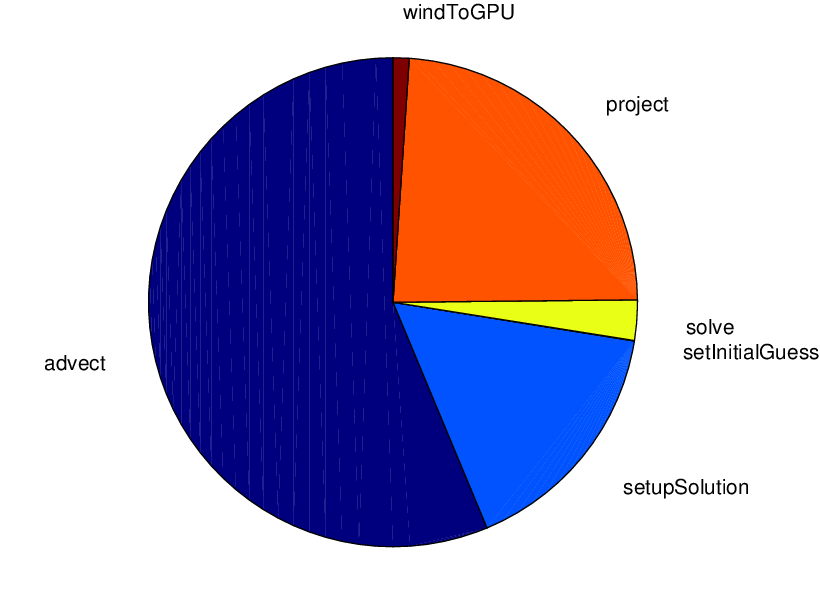
\includegraphics[width=1.0\textwidth]{results/data/td/td_conf3_petsc_gpu}
		\caption{PETSc on the GPU with OpenCL.}
		\label{fig:td_conf3_petsc_gpu}
	\end{subfigure}
	\begin{subfigure}{0.45\textwidth}
		\center
		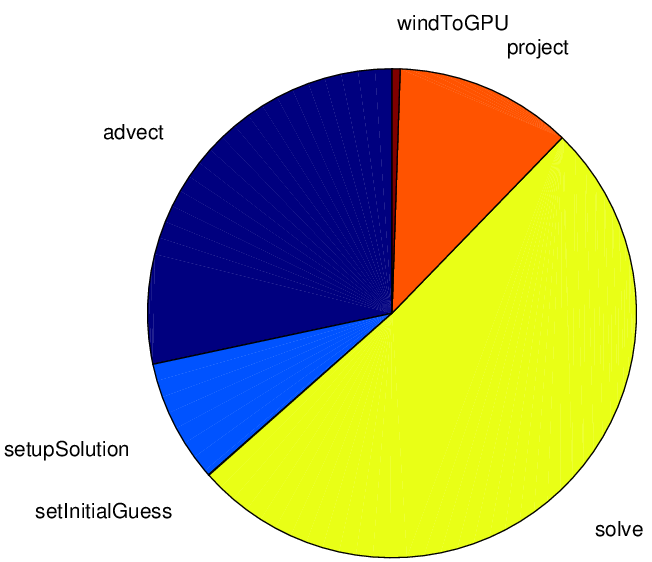
\includegraphics[width=1.0\textwidth]{results/data/td/td_conf3_petsc_cpu}
		\caption{PETSc on the CPU.}
		\label{fig:td_conf3_petsc_cpu}
	\end{subfigure}
	\caption{Compute time benchmark of the execution time of the key functions
			with configuration 3}
	\label{fig:td_conf3}
	
\end{figure}

\begin{figure}[ht]
	\center
	
	\begin{subfigure}{0.45\textwidth}
		\center
		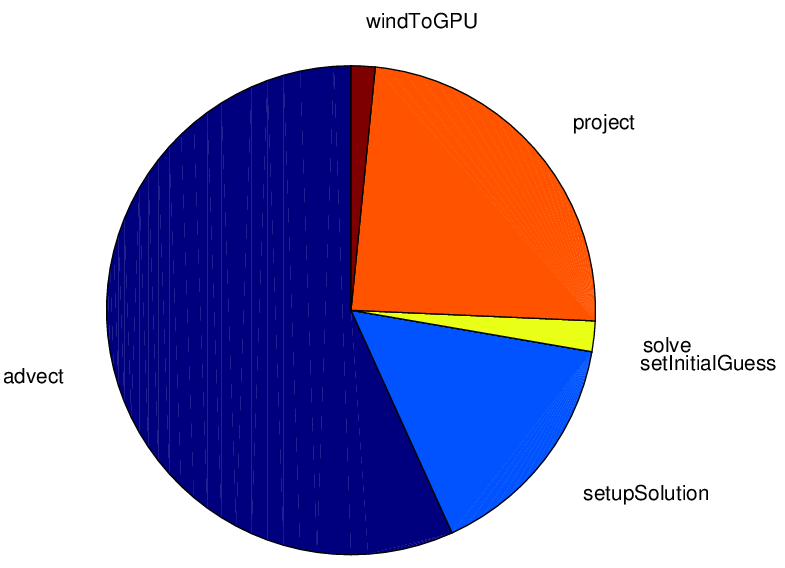
\includegraphics[width=1.0\textwidth]{results/data/td/td_conf4_petsc_gpu}
		\caption{PETSc on the GPU with OpenCL.}
		\label{fig:td_conf4_petsc_gpu}
	\end{subfigure}
	\begin{subfigure}{0.45\textwidth}
		\center
		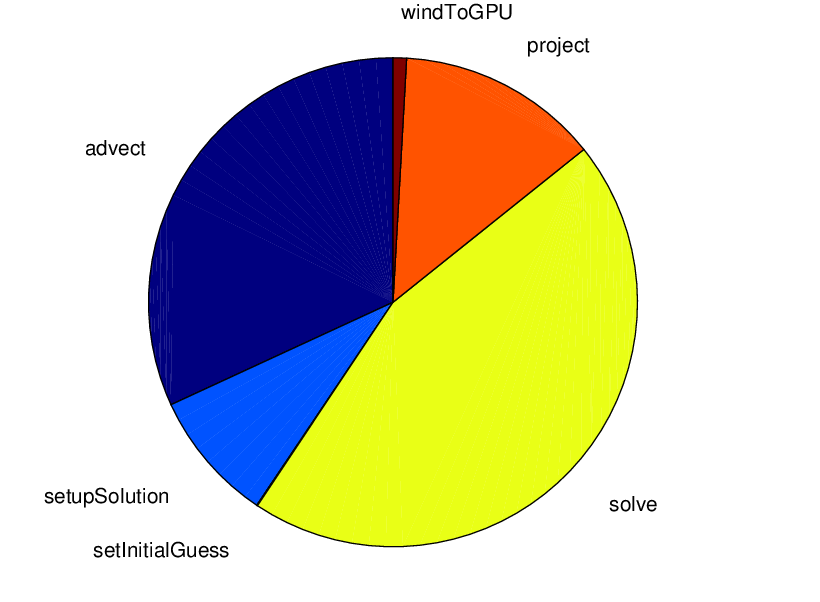
\includegraphics[width=1.0\textwidth]{results/data/td/td_conf4_petsc_cpu}
		\caption{PETSc on the CPU.}
		\label{fig:td_conf4_petsc_cpu}
	\end{subfigure}
	\caption{Compute time benchmark of the execution time of the key functions
			with configuration 4}
	\label{fig:td_conf4}
	
\end{figure}

In the wind simulation benchmarks using PETSc on the CPU only, we see that the
fraction of the wind simulation time spent solving the discretized Poisson
equation is roughly independent of the problem size. As the resolution of the
wind velocity field increases, the fraction of the simulation time spent solving
the Poisson equation remains roughly unchanged. When benchmarking PETSc with the
GPU, the fraction of the execution time spent solving the Poisson equation is
reduced quickly when the problem size increases as the computational power of the
GPU is better utilized for larger problems.

\subsection{Solver Benchmark}

Here the execution time of the Poisson solver is benchmarked. The reason for
only benchmarking the solver is that only the solver uses functions implemented
in PETSc to compute the result, the other functions run on the CPU with a single
thread. As the purpose of this project is to benchmark PETSc's GPU
implementation, benchmarking the functions that don't use PETSc is not within
the scope of the project.

The benchmark measures the execution time of the solver as a function of the
size of the wind field. The execution time of the solver used for the benchmark
is the average execution time after 100 frames of simulation. The following
configurations for the resolution of the wind field was used for this benchmark:

\begin{itemize}
	\item \{32, 16, 32\}
	\item \{32, 32, 32\}
	\item \{64, 32, 64\}
	\item \{64, 64, 64\}
	\item \{128, 64, 128\}
	\item \{128, 128, 128\}
	\item \{256, 128, 256\}
\end{itemize}

The total size of the wind field includes the external boundary points. The
solver methods selected for the benchmark is the conjugate gradient method (CG)
and general minimum residual method (GMRES). Both the CPU and the GPU
implementation of these methods are included in the benchmark. The CG method is
specified with the command line argument "\emph{-ksp\_type cg}" and GMRES is
specified with the argument "\emph{-ksp\_type gmres}". In addition the
successive overrelaxation (SOR) solver implemented in the wind simulator has
been included in the benchmark. The SOR solver has been hand implemented in
CUDA in previous work on the snow simulator performed by other students, the
previous work on the snow simulator is discussed in chapter \ref{chap:prevwork}.
The purpose of including the SOR solver is to compare its performance with the
PETSc solvers.

\begin{figure}[ht]
	\center
	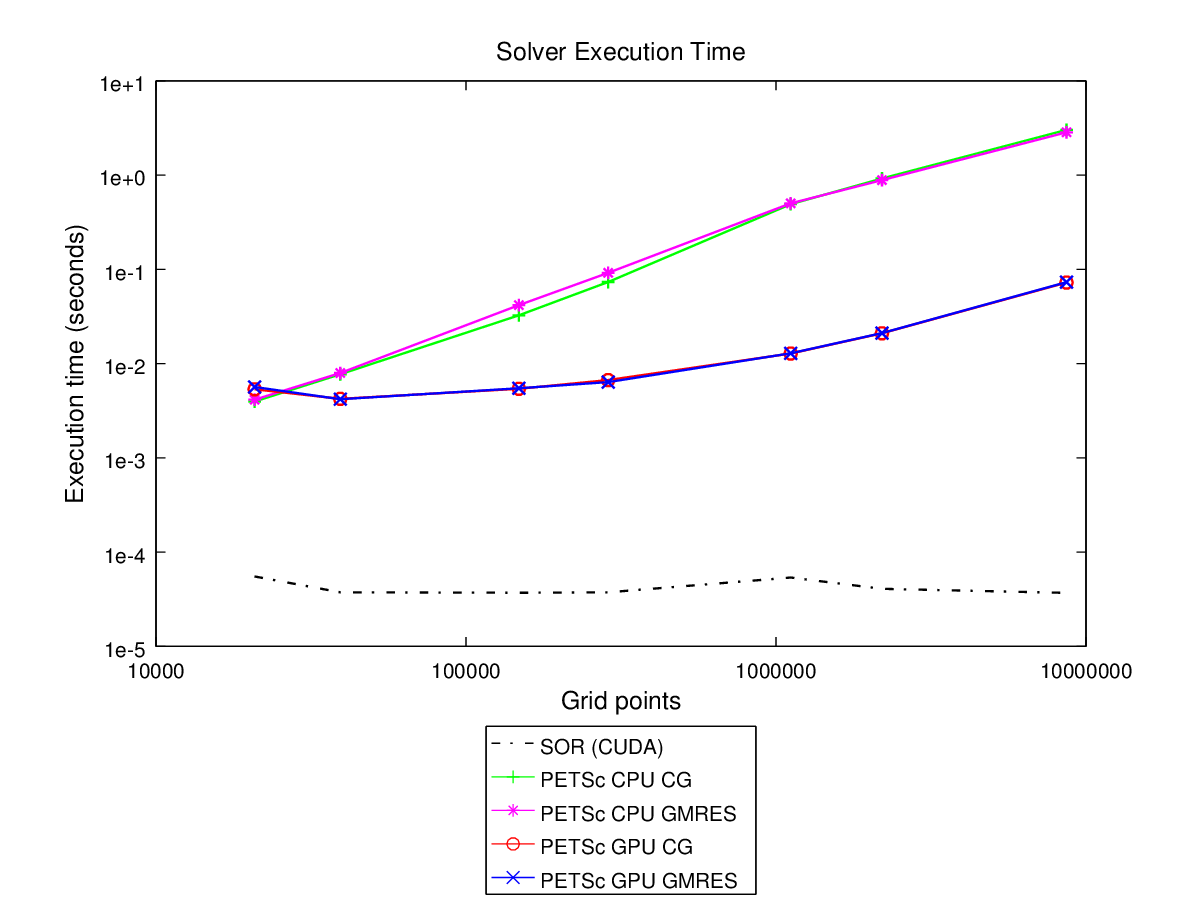
\includegraphics[width=1.0\textwidth]{results/data/sb/exec_time_all}
	\caption{Graph comparing execution time of the different solvers for the
		wind simulator.}
	\label{fig:sb_exec_time_all}
\end{figure}

The results of the solver benchmark is shown in figure \ref{fig:sb_exec_time_all}.
From the graph we see that the hand implemented SOR solver is several orders of
magnitude faster than PETSc solvers and the execution time remains constant.
Another observation is that there is almost no difference in the execution time
and the growth of the execution time when comparing CG and GMRES. Finally we see
that while the GPU implementations of the PETSc solvers have a much slower growth
in their execution time in the beginning than the CPU implementations, but after
passing one million grid points their growth becomes quite similar.

\subsection{Solver Speedup}

In this section the speedup of the GPU implementation of the PETSc solvers will
be benchmarked. The speedup of a solver is defined as $S_p = \frac{T_1}{T_p}$,
where $T_1$ is the execution time of the CPU implementation of the PETSc solver,
and $T_p$ is the execution time of the GPU implementation of the PETSc solver.
The data measurements used here are the same as for the execution time benchmark.

\begin{figure}[ht]
	\center
	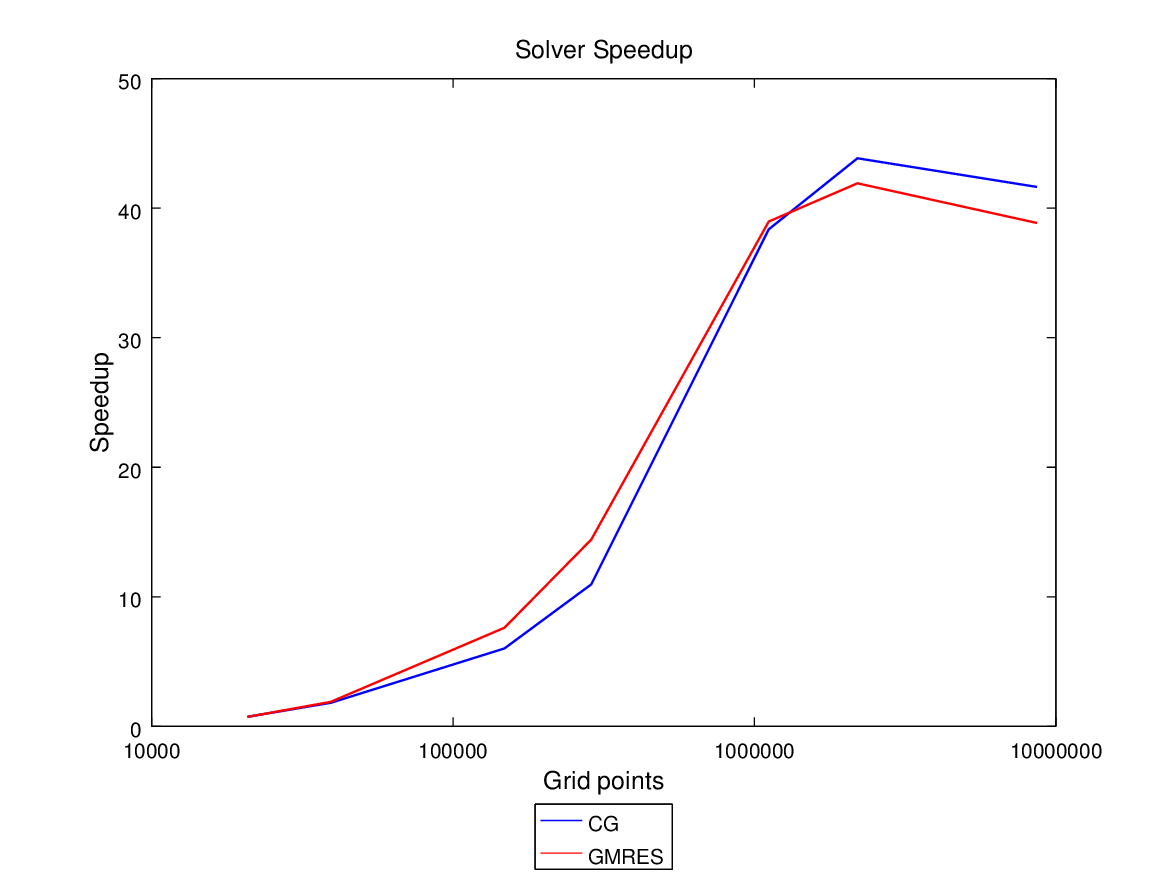
\includegraphics[width=1.0\textwidth]{results/data/sb/speedup_all}
	\caption{Graph showing the speedup of the CG and GMRES methods.}
	\label{fig:speedup_all}
\end{figure}

The results from figure \ref{fig:speedup_all} correlates with the results from
the execution time benchmark, when the problem size reaches one million total
grid points the speedup of the GPU implementation stops growing.
